\chapter{Полученные результаты}

В данной главе будут описаны эксперименты, проведенные для проверки качества и практической применимости алгоритма, и их результаты.
После чего будут даны рекомендации по применению алгоритма и планы его дальнейшего развития.

\section{Результаты экспериментов}
\label{sec:sec_3_1}

В разделе будет описаны проведенные для проверки качества алгоритма эксперименты.

\subsection{Прямой и обратный проход}
Самый простой эксперимент - построить спектрограмму из аудиосигнала, и сразу же преобразовать ее обратно в звук. 
После чего снова построить спектрограмму и сравнить спектрограммы исходного и восстановленного сигнала.

Эксперимент показал, что в случае с сохранением фазы, сигнал восстанавливается точно в области низких частот,
и в зависимости от выбора шага свертки, возможна погрешность в области высоких частот (см. Рисунок \ref{fig:spec_diff_results}).
Сравнение сгенерированных аудиозаписей показало, что человек не слышит этой разницы, что позволяет использовать 
больший шаг свертки, чем необходимый для точного восстановления.

\begin{figure}
  \centering
  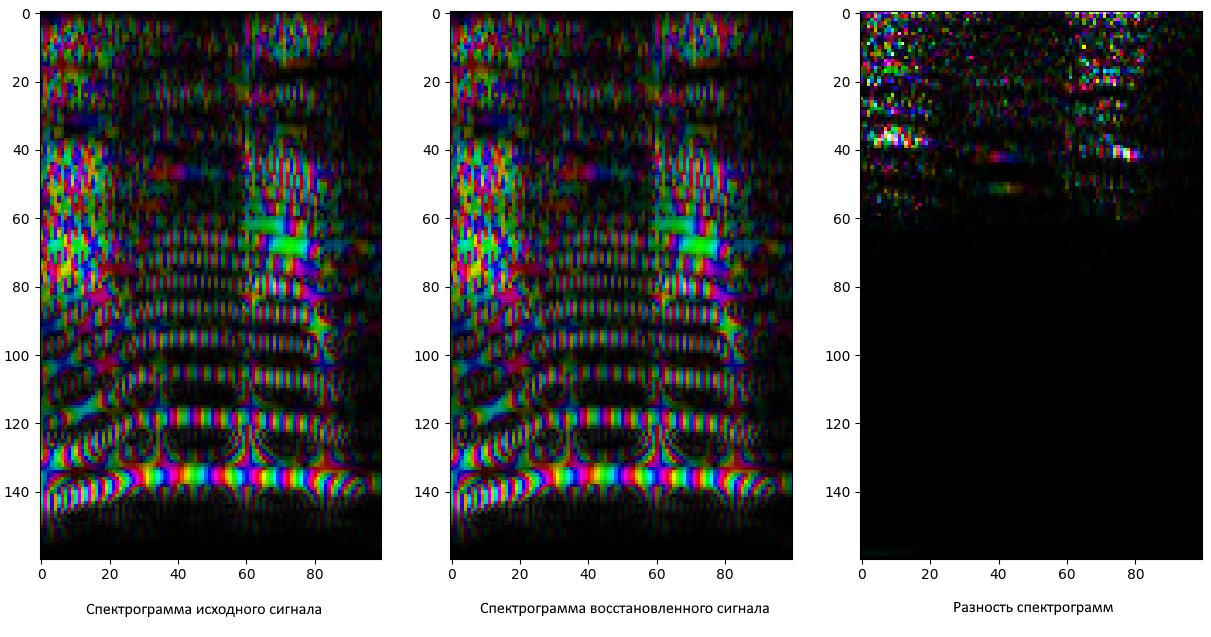
\includegraphics[width=0.8\linewidth]{figures/spec_diff}
  \caption{Спектрограмма сигнала до и после восстановления и их разность}
  \label{fig:spec_diff_results}
\end{figure}

В случае с восстановлением фазы с помощью алгоритма Гриффина-Лима расхождения с исходной спектрограммой присутствуют во всей частотной области
(см. Рисунок \ref{fig:spec_diff_griffinlim}). Но они тоже не слышны человеком, поскольку представляют собой незначительные сдвиги 
отдельных событий по времени в пределах нескольких шагов свертки.

\begin{figure}
  \centering
  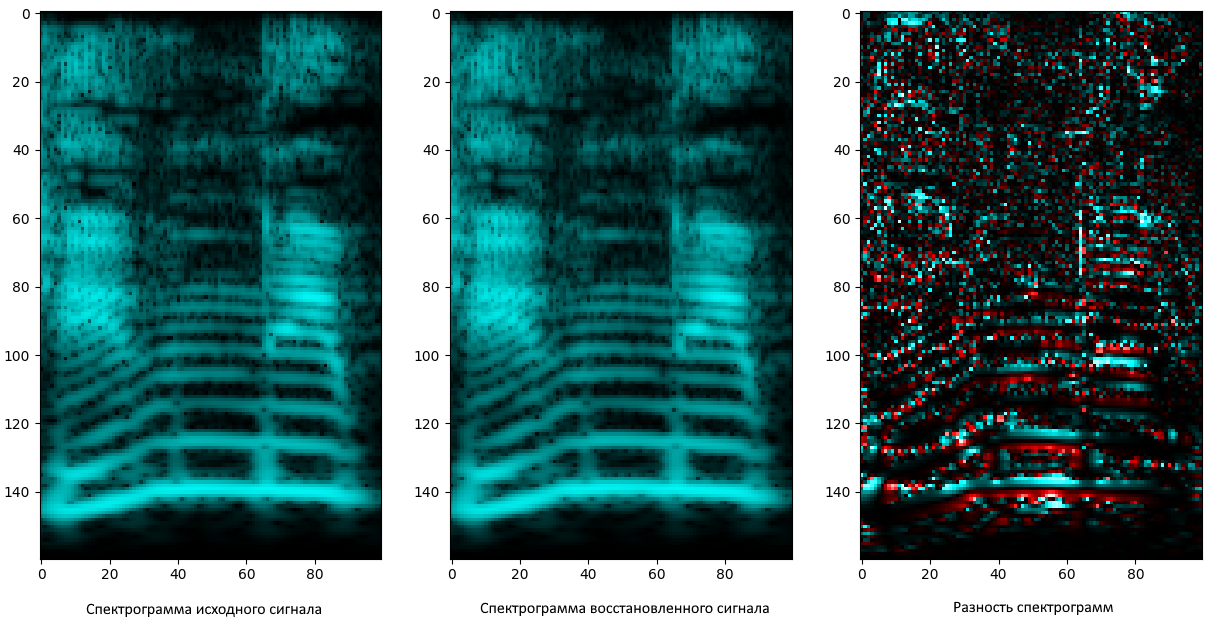
\includegraphics[width=0.8\linewidth]{figures/spec_diff_griffinlim}
  \caption{Спектрограмма сигнала до и после восстановления с реконструкцией фазы и их разность}
  \label{fig:spec_diff_griffinlim}
\end{figure}


\subsection{Устойчивость к трансформациям и искажениям}

Был произведен ряд экспериментов для определения устойчивости преобразования к трансформациям и искажениям. 

Исследовались следующие методы:
\begin{enumerate}[1.]
  \item Вейвлет-преобразование с сохранением фазы
  \item Вейвлет-преобразование с восстановлениме фазы с помощью адаптированного алгоритма Гриффина-Лима
  \item Классический алгоритм STFT и Гриффина-Лима в линейной шкале
\end{enumerate}

После построения спектрограммы она была подвергнута одному из следующих преобразований:
\begin{itemize}
  \item Добавление шума
  \item Сжатие и растяжение по времени
  \item Сжатие и растяжение по частоте
  \item Зануление случайных элементов
  \item Зануление прямоугольных участков
  \item Размытие участков
\end{itemize}

Из полученной спектрограммы восстанавливался аудиосигнал, качество которого сравнивалось с исходным на слух.
Результаты эксперимента приведены в таблице \ref{table:transform_exp}.
Если не было выявлено каких-либо артефактов, в ячейке ставится знак $+$.
Если выявлено незначительное ухудшение качества, ставится знак $\pm$.
Если качество значительно ухудшилось, ставится знак $-$.

\begin{table}[h!]
\centering

\begin{tabular}{||c c c c||} 
 \hline
  Трансформация \textbackslash \  Метод                & Сохр. фазы & Восст. фазы & GriffinLim \\ [0.5ex] 
 \hline\hline
  Добавление шума                      & $+$ & $+$ & $-$ \\
  Сжатие и растяжение по времени       & \pm & $+$ & \pm \\
  Сжатие и растяжение по частоте       & \pm & $+$ & \pm \\
  Зануление случайных элементов        & $+$ & $+$ & $-$ \\
  Зануление прямоугольных участков     & $+$ & $+$ & $-$ \\
  Размытие участков                    & \pm & \pm & $-$ \\ [1ex] 
 \hline
\end{tabular}
\caption{Устойчивость методов восстановления звука к трансформациям и искажениям}
\label{table:transform_exp}
\end{table}

В итоге, предлагаемый метод продемонстрировал ощутимое преимущество с точки зрения устойчивости к искажениям.


\subsection{Нейросетевой автоэнкодер представления с сохранененной фазой}
\label{subsec:keep_phase_net}

Для проверки гипотезы о возможности обучить нейросеть предсказывать сразу комплексное представление спектрограммы была обучена 
несложная нейронная сеть - автоэнкодер на основе архитектуры ResNet с 1D свертками. 
Пространственная размерность в конечном итоге сжималась в 8 раз.
Исходный шаг спектрограммы по времени соответствовал частоте 400 Гц.

В итоге эксперимента был получен следующий результат: Нейросеть смогла обучиться кодировать и декодировать когерентную часть спектрограммы
(гласные, звонкие согласные и т.д.) практически без потерь. Однако, шумоподобные данные (глухие согласные, шипящие) 
были утеряны, то есть, сглажены к нулевому среднему. 

Данный результат приводит к выводу, что подход с сохранением фазы возможен, но требуется отдельно обрабатывать шумоподобные данные: 
предсказывать не конкретную реализацию шума, а его стд. отклонение. Разделять спектрограмму на когерентный сигнал и шум можно как 
снаружи нейросети (как один из этапов преобразования), так и внутри сети 
(например предсказывать плавающее среднее и стд. отклонение, сравнивать их лосс-функцией с этими же параметрами эталона).


\subsection{Обучение Tacotron2 для работы с предлагаемым форматом}

В данном эксперименте была обучена модель синтеза речи Tacotron2 \cite{Tacotron2}. 
Был адаптирован готовый рецепт из open-source проекта Coqui-TTS \cite{coquiTTS}. 
В него была интегрирована реализация предлагаемого алгоритма для построения спектрограммы и восстановления звука.

В результате эксперимента получилась обученная модель, способная генерировать спектрограммы в предлагаемом вейвлет-представлении, 
которые потом декодировались в звук.

В качестве ближайших аналогов, с которыми производилось сравнение, были выбраны две следующие конфигурации:
\begin{itemize}
  \item Tacotron2 + HiFi-Gan - оригинал, обученные веса были заранее доступны в открытом доступе.
  \item Tacotron2 + GriffinLim - ближайший алгоритмический аналог. Ожидается, что по качеству будет заметно хуже первого варианта, и предлагаемый метод будет заметно лучше этого варианта.
\end{itemize}

Далее была произведена оценка качества звука. В качестве метрики для оценивания была выбрана метрика \textbf{Mean Opinion Score}, 
оцениваемая с помощью нейросети DNSMOS (Microsoft) \cite{dnsmos}. 
Выбор данной метрики обусловлен тем, что для ее расчета не требуется оригинал аудиозаписи для сравнения, поэтому ее можно использовать с 
генеративными моделями. Кроме того, она широко используется как одна из метрик качества в современных научных работах и признается научным сообществом.

Изначально, данная метрика оценивалась исходя из усредненной субъективной оценки группы пользователей, 
которым давали прослушать аудиозапись и предлагали выставить оценку качества от 1 до 5. 
Со временем накопилось достаточное количество данных, чтобы обучить нейросетевую модель, 
которая будет предсказывать данную оценку без необходимости собирать группу людей. Данный подход и был использован для оценки качества синтезируемого звука.
Результаты измерений представлены в таблице \ref{table:mos_tacotron}

\begin{table}[h!]
\centering

\begin{tabular}{||m{5cm} c c c||} 
 \hline
  Конфигурация \textbackslash \ Показатель &  Overall MOS & Signal MOS & Backgr. MOS \\ [0.5ex] 
 \hline\hline
  Tacotron2 + HiFi-Gan & 3.19 & 3.49 & 4.02 \\
  Tacotron2 + GriffinLim & 2.77 & 2.95 & 4.11 \\
  Tacotron2 (fine-tuned) + Новый декодер & \textbf{3.28} & \textbf{3.51} & \textbf{4.15} \\ [1ex] 
 \hline
\end{tabular}
\caption{Сравнение качества синтезированного звука по метрике MOS}
\label{table:mos_tacotron}
\end{table}

В результате проведенного эксперимента можно сделать вывод, что предлагаемый метод в сочетании с нейросетями 
позволяет достигать качества звука не хуже, чем нейросетевой декодер (напр. HiFi-Gan).

\section{Наблюдения}
\begin{markdown}
  - рекомендуемые значения параметров
  - как устроена картинка с фазами, когерентный сигнал крутится вдоль времени с частотой сигнала, его след крутится весь на той же самой частоте
  - избыточность информации в шумах, можно заменить сам шум на информацию о распределении шума
  - голос и волны от резонаторов можно разложить на f0 (pitch) и АЧХ резонатора, и перемножать гармоники на АЧХ резонатора, можно будет легко менять pitch.
\end{markdown}

\section{Практическая ценность алгоритма}
\begin{markdown}
   сферы применения алгоритма, польза от него:
    - польза для нейросетей
      - скорость инференса
      - скорость обучения
      - стабильность обучения
      - простота разработки
      - без потери качества
  - сравнение метода с другими вокодерами
    - удобство
    - гибкость
    - универсальность
    - точность
    - скорость
  - примеры работы этого алгоритма и других, сравнение, подсветить недостатки других
\end{markdown}

\section{Планы развития}
\begin{markdown}
 - дальнейшая работа
   - разделение на когерентный сигнал и шум (в шуме хранится больше информации чем нужно, нужно сохранять только распределение, а не реализацию)
   - голос и волны от резонаторов можно разложить на f0 (pitch) и АЧХ резонатора, и перемножать гармоники на АЧХ резонатора, можно будет легко менять pitch.
   - реализация быстрого алгоритма на ускорителях
   - внедрение в существующие модели text-to-speech
\end{markdown}

\section{Выводы по главе}